\subsection{Sq電流}

Sq(Solar quiet)電流とは、太陽静穏時の地磁気日変化を引き起こす電流系であり、主に太陽輻射による電離圏の電気伝導度変化と熱圏風によるダイナモ作用によって駆動される。
Sq電流系は、北半球では反時計回り、南半球では時計回りの渦状構造を持ち、昼間側で極向き（赤道域）の電流成分が卓越する。
\citeauthor{Rastogi1994} \citeyear{Rastogi1994} は、低緯度地域における地磁気H成分の季節変化を解析し、Sq電流系の強度が季節によって変動することを報告している。
特に、電流渦の中心位置や強度が季節変化し、一般に夏半球で電流強度が強まる傾向があることが知られている。
しかしながら、地域的な特性や半球間の非対称性も存在し、例えば南半球の冬至（J-solstice）においてはSq電流系が弱まる傾向が報告されている。

\begin{figure}[htbp]
  \centering
  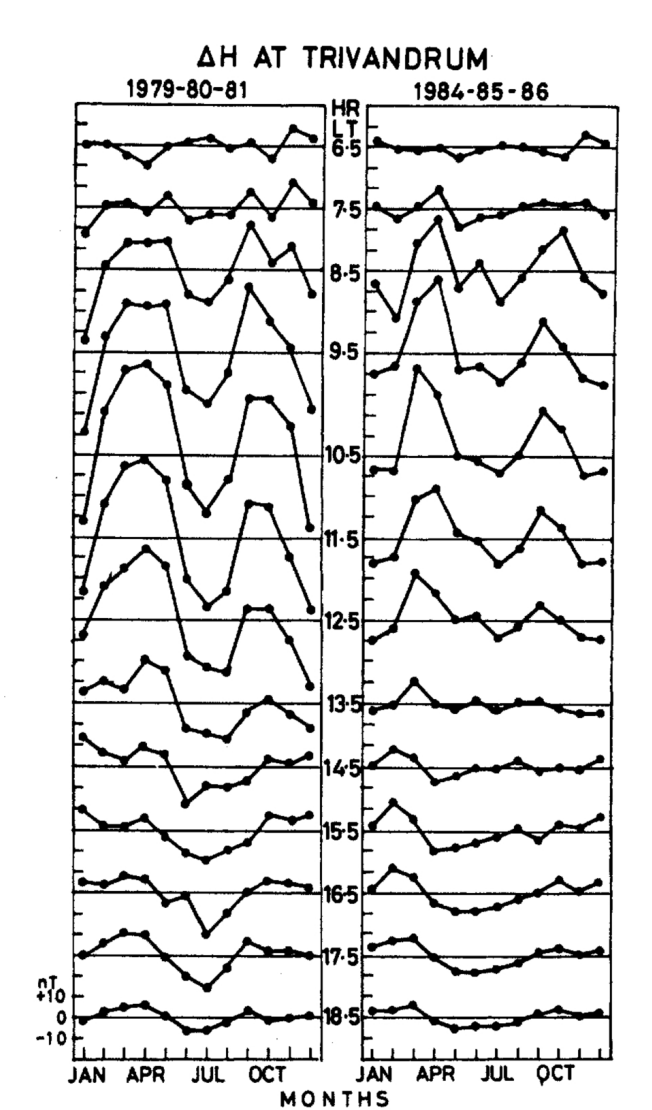
\includegraphics[width=0.8\linewidth]{figures/rastogi_sq.png}
  \caption{Seasonal variations of Sq current system \cite{Rastogi1994}.}
  \label{fig:rastogi_sq}
\end{figure}



